% \documentclass[10pt,draft]{beamer}
\documentclass[10pt]{beamer}

\usetheme{metropolis}
\usepackage{appendixnumberbeamer}
\usepackage{tikz}
\usetikzlibrary{decorations.pathreplacing}
\usepackage{caption}
\usepackage{graphicx}
\usepackage{multirow}
\usepackage{listings}
\usepackage{booktabs}
\usepackage{minted}
\usepackage{algorithm}
\usepackage[noend]{algpseudocode}
\pgfdeclarelayer{bg}    % declare background layer
\pgfsetlayers{bg,main}  % set the order of the layers (main is the standard layer)
\usepackage{pgfplots}
\usepgfplotslibrary{dateplot}

\usepackage{booktabs}
\usepackage[scale=2]{ccicons}
\usepackage{adjustbox}

\usepackage{xspace}
\newcommand{\themename}{\textbf{\textsc{metropolis}}\xspace}
\usepackage{natbib}
\usepackage{color}
\newcommand{\todo}[1]{\textbf{\textcolor{red}{#1}}}
\def\stackplotStart{2013-12-21} 
\def\stackplotEnd{2018-12-19} 

\title{A Deep Dive into Bitcoin Mining Pools}
\subtitle{An Empirical Analysis of Mining Shares}

\author[shortname]{\textbf{Matteo Romiti} \inst{1}\and
Aljosha Judmayer \inst{2} \\ \and
Alexei Zamyatin \inst{2}\textsuperscript{,} \inst{3} \and
Bernhard Haslhofer \inst{1}}


\institute[shortinst]{\inst{1} Austrian Institute of Technology \and
\inst{2} SBA Research \and \inst{3} Imperial College London}

% \date{\today}

\begin{document}

\maketitle

\begin{frame}[fragile]{Introduction}
    Why do we care about miners?
    \begin{itemize}
        \item Miners decide which transactions to include in a block
        \item Miners decide which blocks to include in the chain
        \item Miners are rewarded with new coins and transaction fees
        \item Miners secure the network (Proof-of-Work algorithm)
        \item Miners can attack the network (e.g., double-spend)
    \end{itemize}
\end{frame}

\begin{frame}[fragile]{Introduction}
    What about Mining Pools?
    \begin{itemize}
        \item Solo mining is not profitable anymore
        \item Miners join pools for steadier revenues
        \item Pools compete to create blocks and claim the rewards
        \item Pool managers coordinate work and rewards among members
    \end{itemize}
\end{frame}

\begin{frame}[fragile]{Research Questions} 
    \begin{enumerate}
        \item How did the mining distribution evolve over time? How can we attribute blocks to mining pools? 
        \item How do mining pools distribute rewards? How can we detect payments to pool members?
        \item How decentralized is a mining pool? Who are the pool members? What's their behavior?
    \end{enumerate}
\end{frame}

\section{Background} 
\begin{frame}[fragile]{Background | Coinbase Flow}
    \begin{figure}
        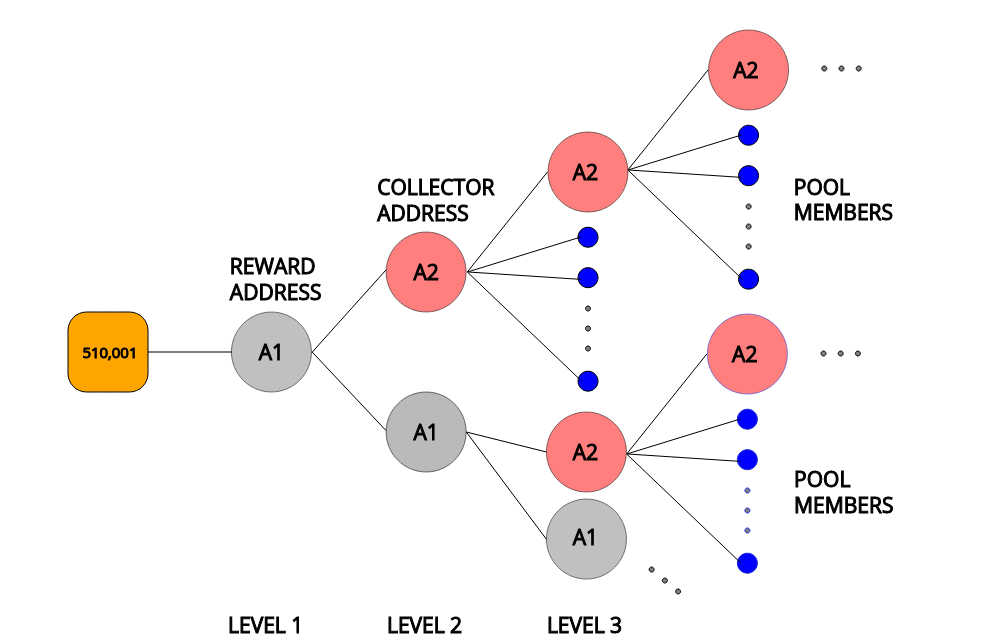
\includegraphics[width=.8\textwidth]{images/flow_example.png}
        \\Example of a coinbase flow
    \end{figure}
\end{frame}

\begin{frame}[fragile]{Background | Coinbase Flow}
    \begin{figure}
        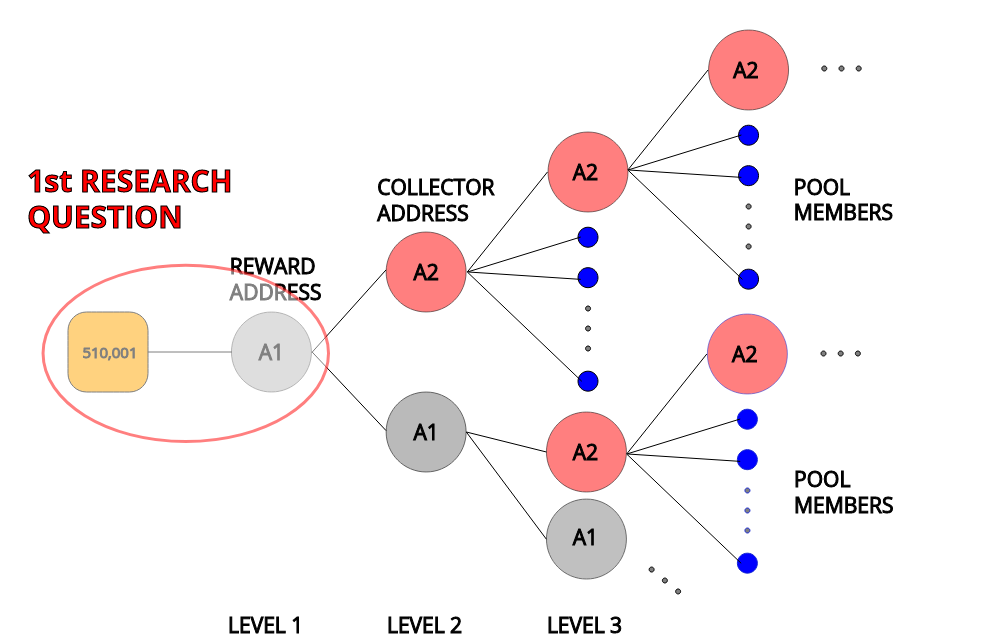
\includegraphics[width=.8\textwidth]{images/1rq.png}
        \\Example of a coinbase flow
    \end{figure}
\end{frame}

\begin{frame}[fragile]{Background | Coinbase Flow}
    \begin{figure}
        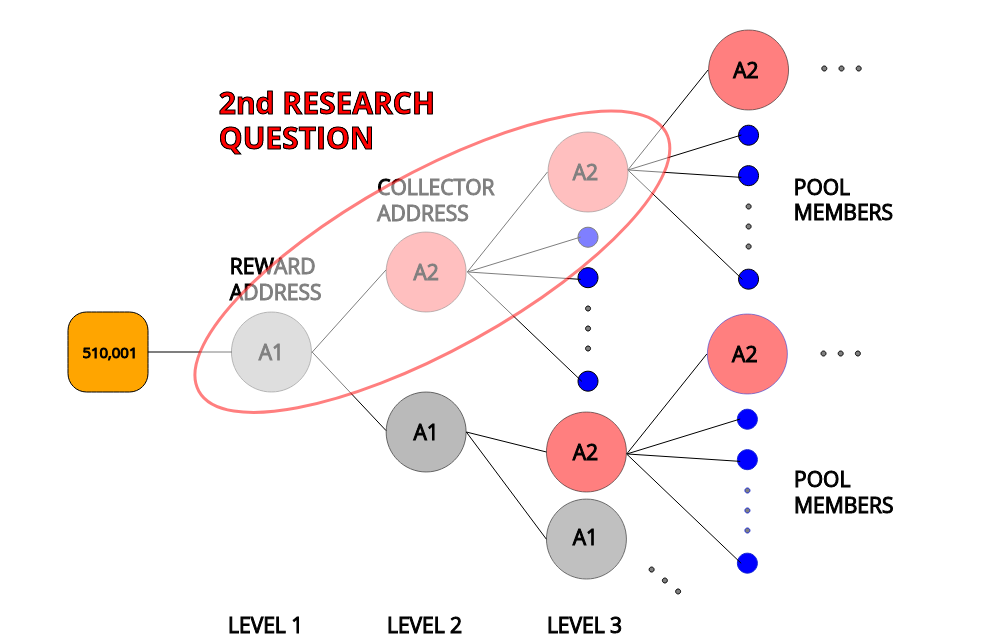
\includegraphics[width=.8\textwidth]{images/2rq.png}
        \\Example of a coinbase flow
    \end{figure}
\end{frame}

\begin{frame}[fragile]{Background | Coinbase Flow}
    \begin{figure}
        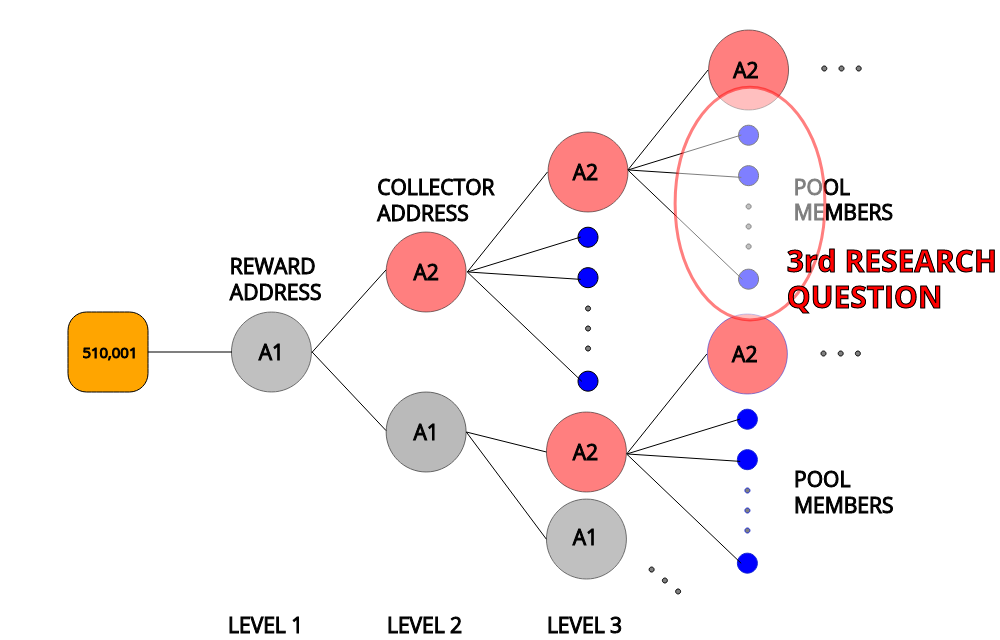
\includegraphics[width=.8\textwidth]{images/3rq.png}
        \\Example of a coinbase flow
    \end{figure}
\end{frame}

\begin{frame}[fragile]{Background | Multiple-Input Clustering Heuristic}
    \begin{figure}
        \centering
        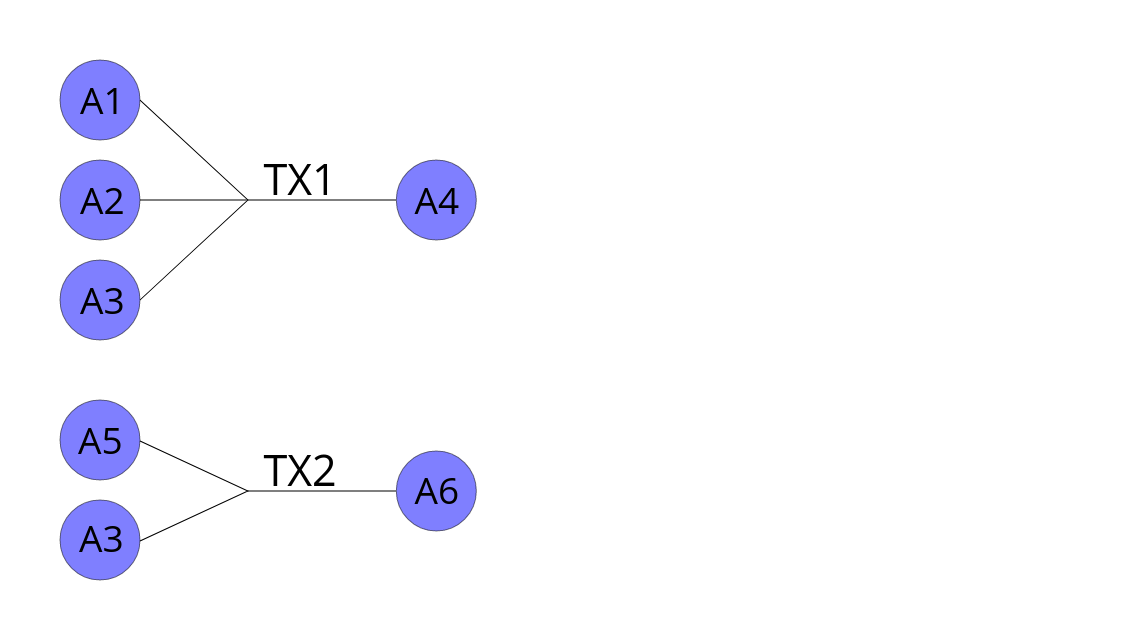
\includegraphics[width=0.9\textwidth]{images/clustering1.png}
        \\Multiple-input clustering heuristic
    \end{figure}
\end{frame}

\begin{frame}[fragile]{Background | Multiple-Input Clustering Heuristic}
    \begin{figure}
        \centering
        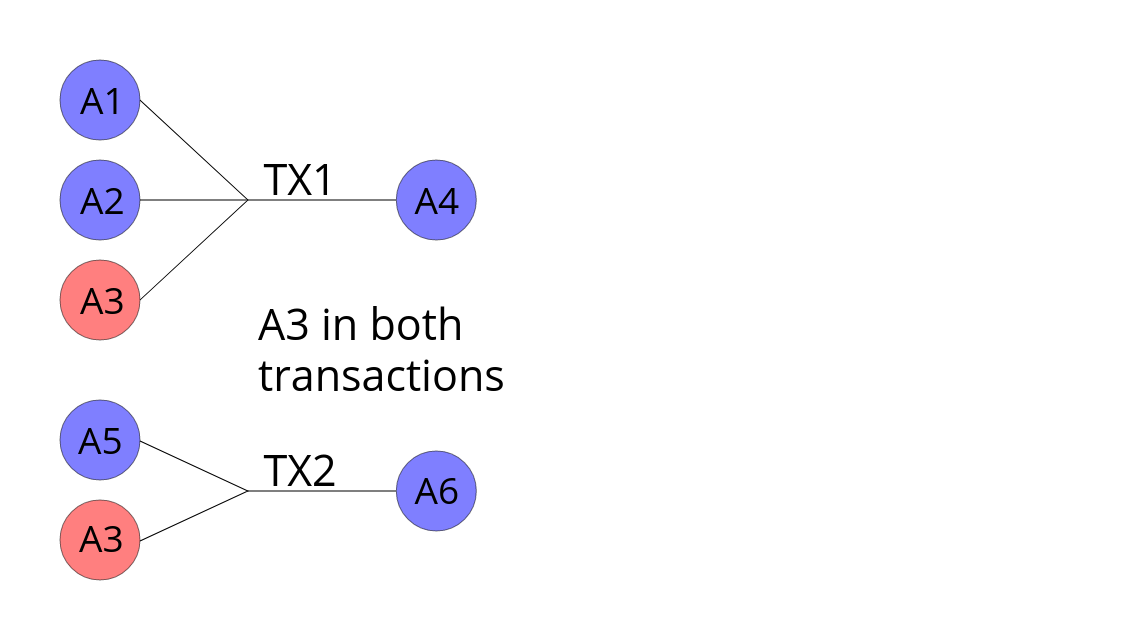
\includegraphics[width=0.9\textwidth]{images/clustering2.png}
        \\Multiple-input clustering heuristic
    \end{figure}
\end{frame}

\begin{frame}[fragile]{Background | Multiple-Input Clustering Heuristic}
    \begin{figure}
        \centering
        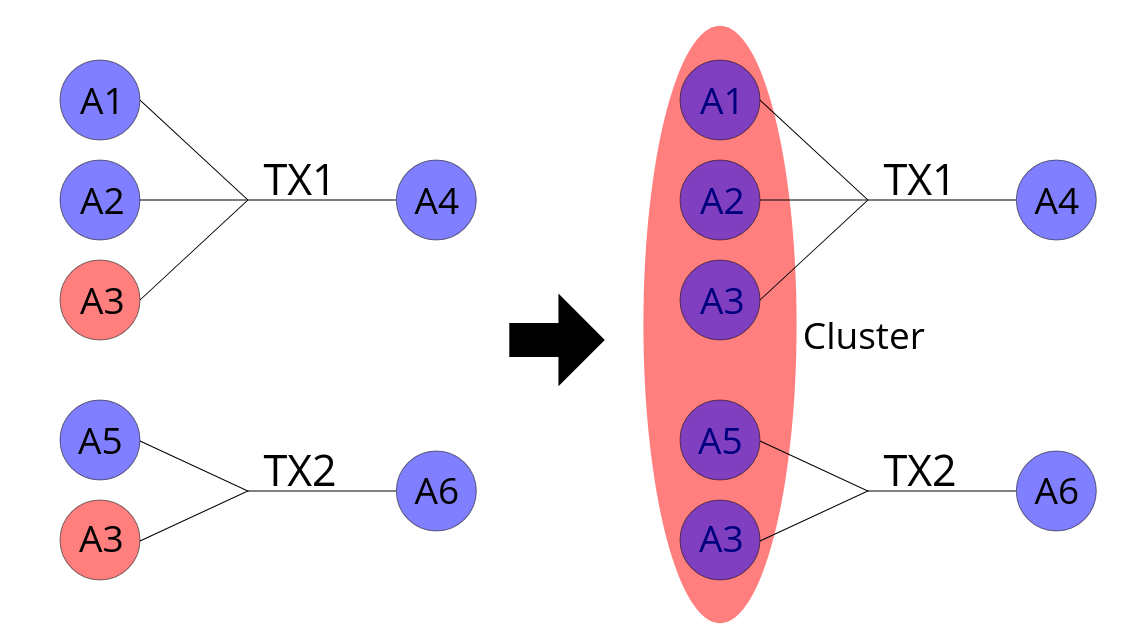
\includegraphics[width=0.9\textwidth]{images/clustering3.png}
        \\Multiple-input clustering heuristic
    \end{figure}
\end{frame}

\begin{frame}[fragile]{Background | Multiple-Input Clustering Heuristic}
    \begin{figure}
        \centering
        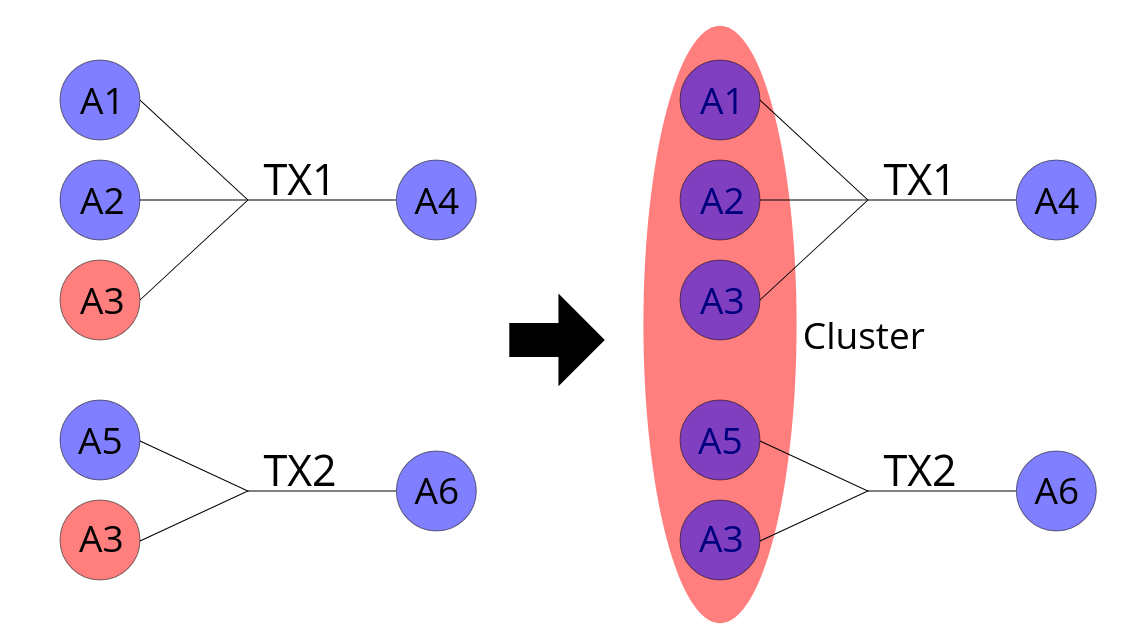
\includegraphics[width=0.9\textwidth]{images/clustering3.png}
    \end{figure}
    \begin{figure}
        \centering
        \def\svgwidth{\columnwidth}
        \input{images/graphsense.pdf_tex}
    \end{figure}
\end{frame}

\section{Block Attribution} 
\begin{frame}[fragile]{Block Attribution | Data Sources}
    \begin{itemize}
        \item Blocktrail API (till block 514239, March 2018)
        \item Blockchain.info Github repository
        \item BTC.com Github repository
        \item Walletexplorer.com's tags with multiple-input clustering heuristic (GraphSense)
        \item Coinbase markers manually retrieved
    \end{itemize}
\end{frame}

\begin{frame}[fragile]{Block Attribution | Methodology}
    \begin{figure}
        % \centering
        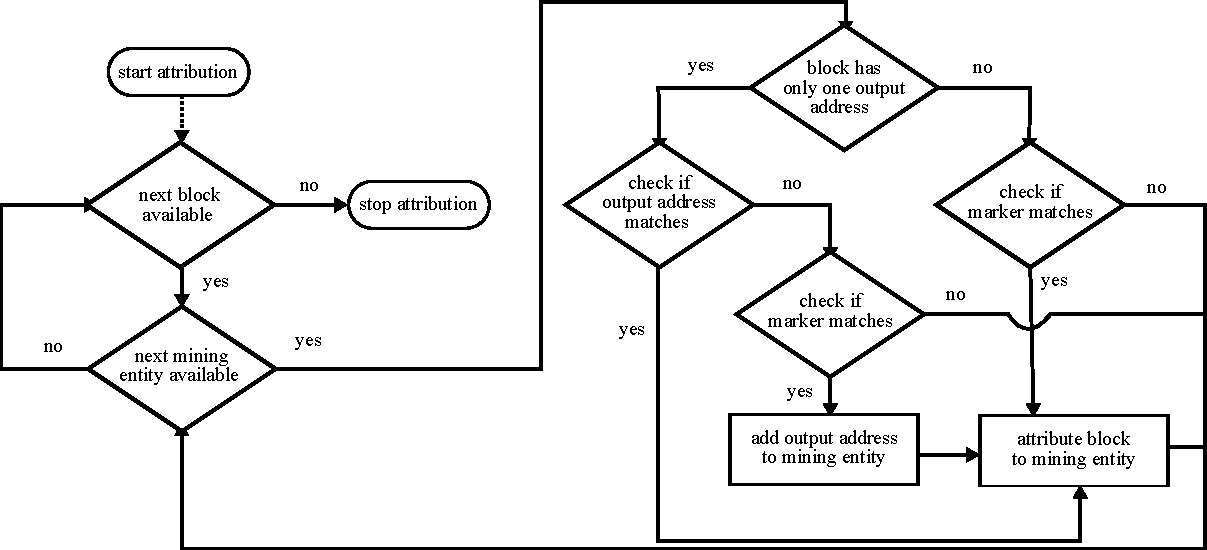
\includegraphics[width=\textwidth]{images/attribution_horizontalized.pdf}
        \caption{High level flow chart representing our attribution scheme.}
        \label{fig:attribution}
    \end{figure}
\end{frame}

\begin{frame}[fragile]{Block Attribution | Results: Conflicts}
    \setlength{\tabcolsep}{2pt}
    \begin{table}
        \caption{684 attribution conflicts out of 556400 blocks (0.0012\%). From 500,000 to 556,400, we attributed 96.5\% of the blocks (blockchain.info 92\%, $\sim$ 32,100 BTC difference)}\label{tbl:conflicts}
        \scalebox{.9}{
            \begin{tabular}{@{}llll@{}}
            \toprule
            Miner 1       & Miner 2         & Number of conflicts & Example blocks         \\
            \midrule
            BTC.TOP       & CANOE           & 338                 & 516210, 516275, \ldots   \\
            Bixin         & TangPool        & 142                 & 339210, 339284, \ldots    \\
            BTC.com       & Waterhole       & 113                 & 478230, 478328, \ldots    \\
            BTC.TOP       & WAYI.CN         & 81                  & 509073, 509100, \ldots    \\
            ViaBTC        & Okminer         & 5                   & 510279, 523217,        \\
            Yourbtc       & OzCoin          & 3                   & 159846, 159929, 159964 \\
            BitcoinRussia & Bitcoin-Ukraine & 1                   & 524045                 \\
            F2Pool        & BTCC Pool       & 1                   & 482886                 \\
            \bottomrule
            \end{tabular}
        }
    \end{table}
\end{frame}

\begin{frame}[fragile]{Block Attribution | Results: Mining Shares}
    \vspace*{-0.77cm}
    \begin{figure}
        \hspace*{-1.7cm}
        \includegraphics[width=1.23\textwidth]{images/stackplot_periodLen_2016secs_end_554399_numPeriods_138_threshold_4_groupBy_miner.pdf}
        \caption{Evolution of mining pools market shares (\stackplotStart~to \stackplotEnd).}
        \label{fig:stack_miners}
    \end{figure}
\end{frame}

\section{Payout Patterns} 
\begin{frame}[fragile]{Payout Patterns | Data Sources}
    \begin{itemize}
        \item Output of the block attribution procedure to select BTC.com, AntPool and ViaBTC blocks
        \item Blockchain.info API to retrieve coinbase flows
        \item GraphSense to detect exchanges
    \end{itemize}
\end{frame}

\begin{frame}[fragile]{Payout Patterns | Methodology: BTC.com}
    \begin{figure}
        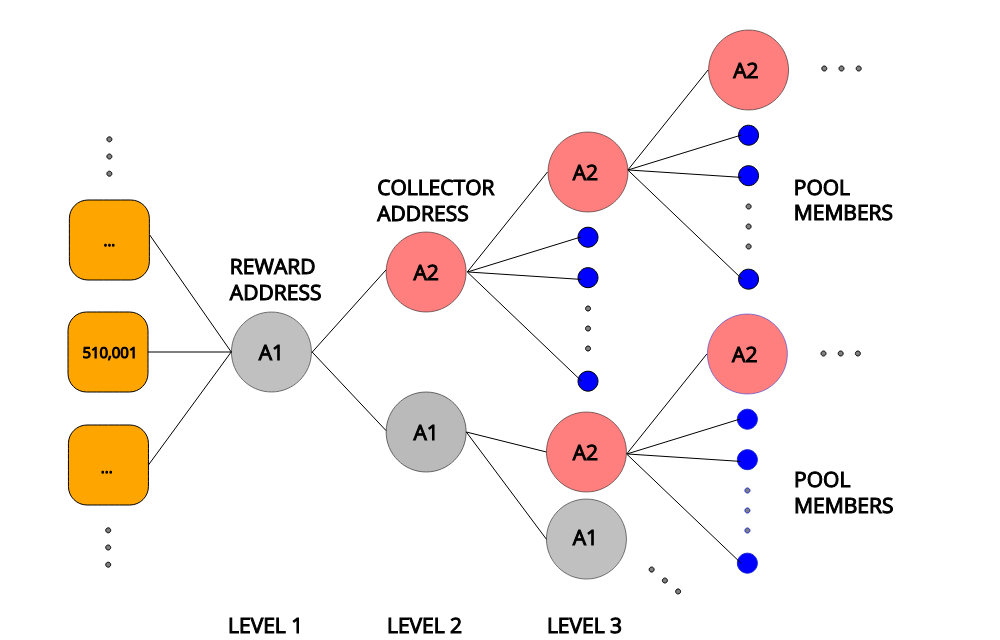
\includegraphics[width=.8\textwidth]{images/flow_BTCcom_example1.png}
        \caption{BTC.com payout pattern observed between block 510,000 and 514,032. In gray: reward addresses, in red: addresses performing payout transactions, in blue: pool members, in green: change addresses. Rounded squares are coinbases of blocks mined by the pool.}
        \label{fig:flow_example}
    \end{figure}
\end{frame}

\begin{frame}[fragile]{Payout Patterns | Methodology: AntPool}
    \begin{figure}
        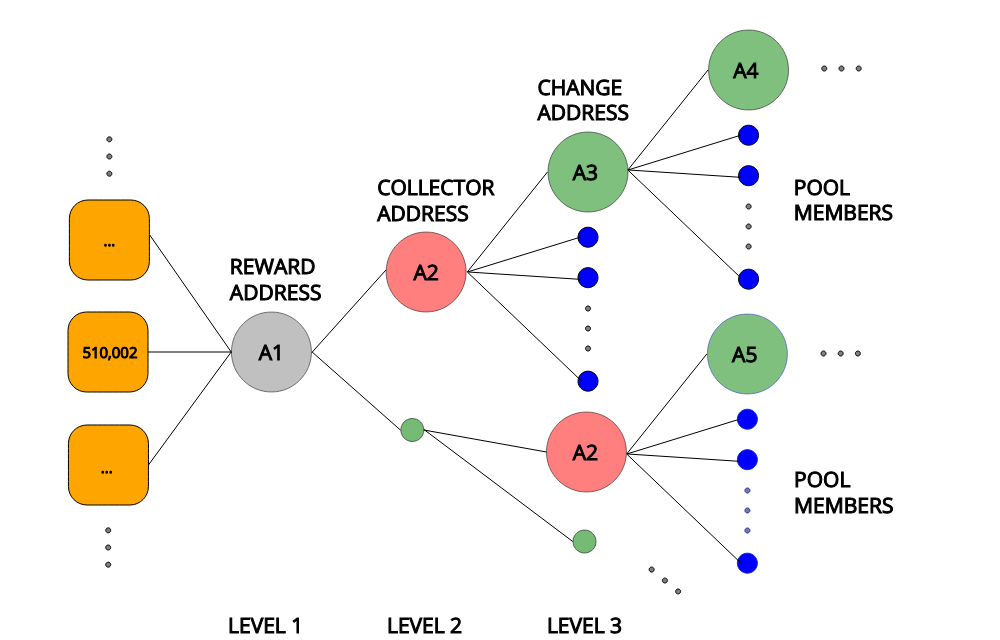
\includegraphics[width=.8\textwidth]{images/flow_AntPool_example1.png}
        \caption{AntPool payout pattern observed between block 510,000 and 514,032. In gray: reward addresses, in red: addresses performing payout transactions, in blue: pool members, in green: change addresses. Rounded squares are coinbases of blocks mined by the pool.}
        \label{fig:antpool_flow}
    \end{figure}
\end{frame}

\begin{frame}[fragile]{Payout Patterns | Methodology: ViaBTC}
    \begin{figure}
        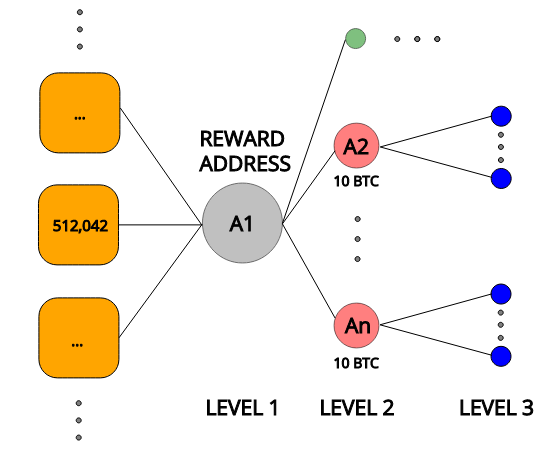
\includegraphics[width=.5\textwidth]{images/flow_ViaBTC_example2.png}
        \caption{ViaBTC payout pattern observed between block 510,000 and 514,032. In gray: reward addresses, in red: addresses performing payout transactions, in blue: pool members, in green: change addresses. Rounded squares are coinbases of blocks mined by the pool.}
        \label{fig:viabtc_flow}
    \end{figure}
\end{frame}

\begin{frame}[fragile]{Payout Patterns | Results}
    \setlength{\tabcolsep}{2pt}
    \begin{table}
        \centering
        \caption{Statistics of retrieved data between block 510,000 and 514,032 ($\sim$ 4 weeks). $N_{B}$: number of blocks mined by the pool, $N_{TX}$: number of identified payout transactions, $N_{A}$: number of identified members' addresses, $N_{C}$: number of identified clusters, $BTC_{M}$: BTC mined by the pool, $BTC_{P}$: BTC paid to pool members (addresses), $\mu$: median value of address reuse.}\label{miners_stats}
        \scalebox{0.95}{
            \begin{tabular}{@{}lrrrrrrrrrr@{}}
                \toprule
                Pool Name & 
                $N_{B}$ & 
                $N_{TX}$ & 
                $N_{A}$ & 
                $N_{C}$ & 
                $BTC_{M}$ &
                $BTC_{P}$ &
                $\dfrac{BTC_{P}}{BTC_{M}}$ & 
                $\mu$ &
                $\dfrac{\mu}{N_A}$ \\
                \midrule
                BTC.com     &1,020  &225    &20,444 &8,900  &13,059 &12,057 &92\%   &20 &9.8 $\times10^{-4}$ \\
                AntPool     &617    &408    &14,166 &5,082  &7,887  &2,333  &30\%   &2 &1.4 $\times10^{-4}$\\
                ViaBTC      &457    &104    &7,171  &3,121  &5,841  &4,284  &75\%   &5 &7.0 $\times10^{-4}$\\
                \bottomrule
            \end{tabular}   
        }
    \end{table}
\end{frame}

\section{Pools Members} 
\begin{frame}[fragile]{Pools Members | Data Sources}
    \begin{itemize}
        \item Output of the block attribution procedure
        \item Output of the payout patterns
        \item Walletexplorer.com + multiple-input clustering heuristic (GraphSense)
    \end{itemize}
\end{frame}

\begin{frame}[fragile]{Pools Members | Results: Cross-Pool Mining}
    \setlength{\tabcolsep}{3pt}
    \begin{table}
        \caption{Cross-pool mining between block 510,000 and 514,032 ($\sim$ 4 weeks), including how much BTC from each pool has been received by those common addresses.} \label{table:crosspool_addresses}
        \scalebox{.95}{
            \begin{tabular}{@{}llllll@{}}
            \toprule
            Pool 1  & Pool 2  & \begin{tabular}[c]{@{}l@{}}Addresses \\ in common\end{tabular} & \begin{tabular}[c]{@{}l@{}}Clusters \\ in common\end{tabular} & \begin{tabular}[c]{@{}l@{}}BTC from\\ Pool 1\end{tabular} & \begin{tabular}[c]{@{}l@{}}BTC from\\ Pool 2\end{tabular} \\ \midrule
            BTC.com & AntPool & 537 (1.58\%) & 434 (3.2\%)        & 664.3 (5.5\%)                                               & 176.8 (7.6\%)                                                \\
            AntPool & ViaBTC  & 115 (0.54\%) & 196  (2.4\%)      & 11.1  (0.47\%)                                               & 102.6 (2.4\%)                                                \\
            ViaBTC  & BTC.com & 250 (0.91\%)  & 267  (2.3\%)     & 175.4 (4.1\%)                                               & 174.1 (1.4\%)                                               \\ \bottomrule
            \end{tabular}
        }
    \end{table}
\end{frame}

\begin{frame}[fragile]{Pools Members | Results: Main Entities}
    \setlength{\tabcolsep}{2pt}
    \begin{table}
        \caption{Cross-pool mining at a cluster level in the time period between block 510,000 and 514,032 ($\sim$ 4 weeks). W: wallet provider, E: exchange service, P: known mining pool, M: unknown mining entity.}\label{table:crosspool_entities}
        \scalebox{0.65}{
            \begin{tabular}{@{}llrrrrrrrrrr@{}}
            \toprule
                          &  & \multicolumn{3}{c}{BTC.com}   & \multicolumn{3}{c}{AntPool}   & \multicolumn{3}{c}{ViaBTC}    &  \\ \cmidrule(lr){3-5} \cmidrule(lr){6-8} \cmidrule(lr){9-11}
            Entity/Actor             & Service        & BTC     & \%BTC & \#Addr. & BTC     & \%BTC & \#Addr. & BTC     & \%BTC & \#Addr. & Total BTC \\ \midrule
            Unknown             & ?       & 8930.39 & 74.07 & 13286       & 1682.25 & 72.09 & 8888        & 2877.02 & 67.17 & 4845        & 13489.67  \\ 
            Bixin               & W+E+P   & 1663.75 & 13.80 & 1061        & 241.28  & 10.34 & 546         & 795.36  & 18.57 & 476         & 2700.39   \\ 
            Huobi.com         & E       & 808.64  & 6.71  & 964         & 142.04  & 6.09  & 759         & 225.50  & 5.27  & 322         & 1176.19   \\ 
            % Old mining clusters & M       & 426.72  & 3.54  & 3793        & 141.84  & 6.08  & 3081        & 300.62  & 7.02  & 1033        & 869.19    \\ 
            Bittrex.com         & E       & 83.71   & 0.69  & 348         & 29.56   & 1.27  & 251         & 43.36   & 1.01  & 177         & 156.63    \\ 
            Xapo.com            & W       & 26.96   & 0.22  & 94          & 70.75   & 3.03  & 64          & 5.79    & 0.14  & 33          & 103.50    \\ 
            Poloniex.com        & E       & 42.65   & 0.35  & 381         & 11.52   & 0.49  & 268         & 19.97   & 0.47  & 139         & 74.15     \\ 
            Luno.com            & W+E     & 36.59   & 0.30  & 258         & 4.06    & 0.17  & 104         & 4.39    & 0.10  & 60          & 45.04     \\ 
            Bitstamp.net        & E       & 8.94    & 0.07  & 57          & 3.55    & 0.15  & 38          & 3.91    & 0.09  & 22          & 16.39     \\ 
            Cryptonator.com     & W+E     & 5.75    & 0.05  & 80          & 0.70    & 0.03  & 41          & 2.70    & 0.06  & 33          & 9.15      \\ 
            BitoEX.com          & W       & 5.09    & 0.04  & 23          & 1.12    & 0.05  & 35          & 2.19    & 0.05  & 4           & 8.39      \\ 
            CoinHako.com        & W+E     & 3.59    & 0.03  & 4           & 0.29    & 0.01  & 3           & 0.24    & 0.01  & 2           & 4.12      \\ 
            Bitcoin.de          & E       & 1.86    & 0.02  & 26          & 0.76    & 0.03  & 13          & 0.58    & 0.01  & 7           & 3.19      \\ \bottomrule
            \end{tabular}
        }
    \end{table} 
\end{frame}

\begin{frame}[fragile]{Pools Members | Results: Pool Centralization}
    \begin{figure}
        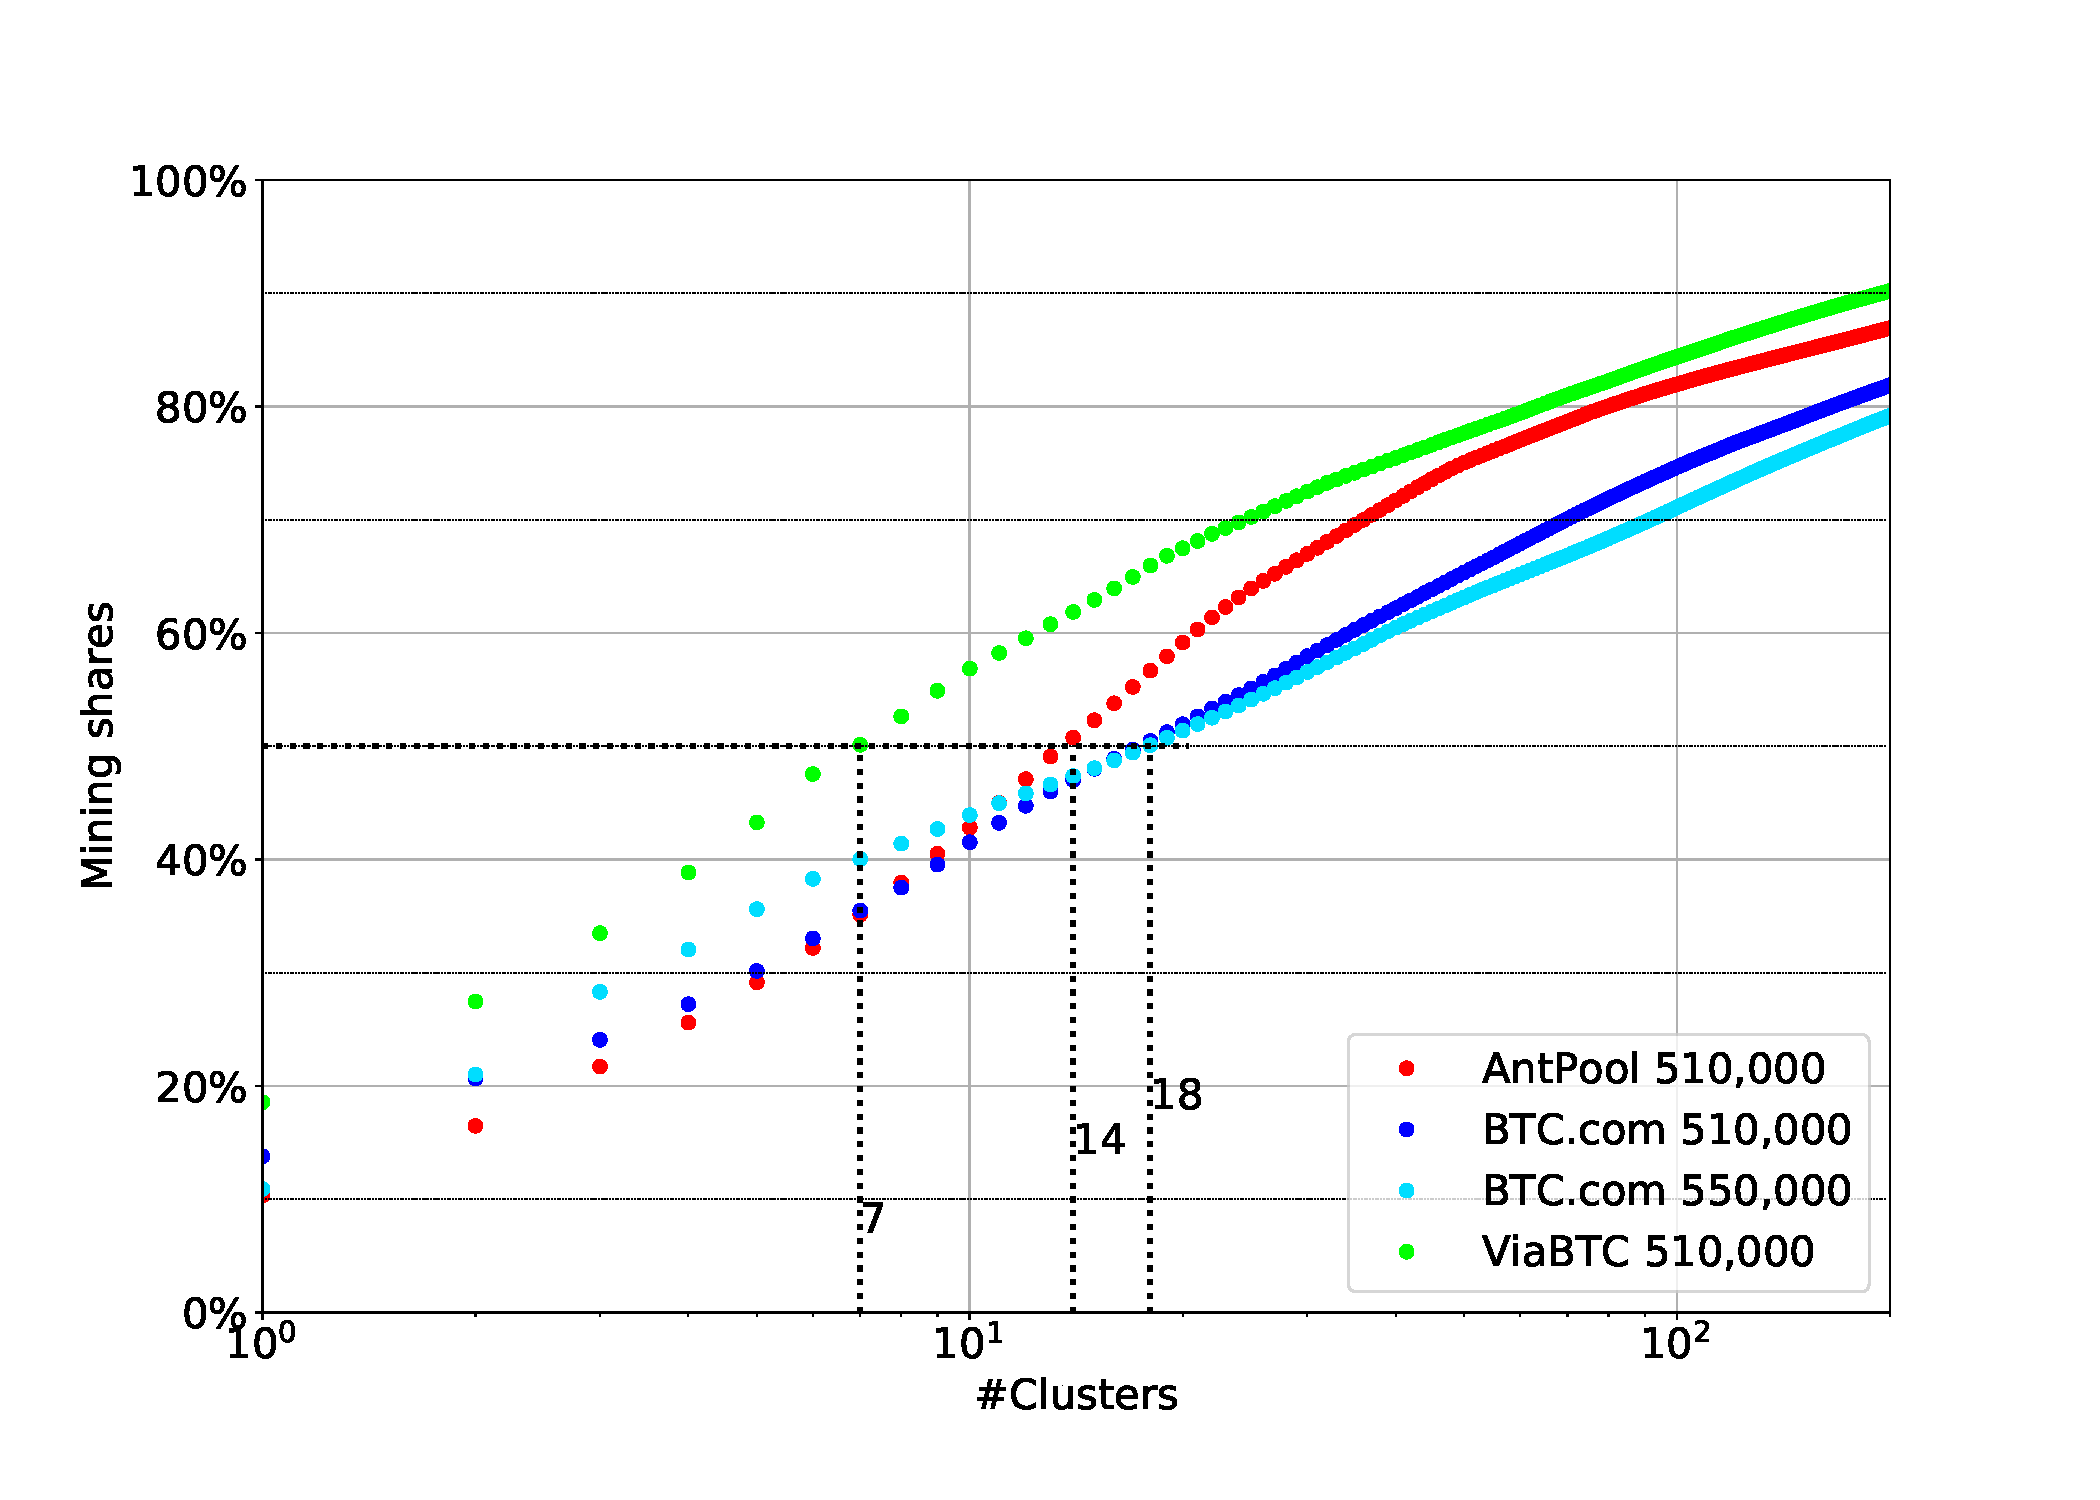
\includegraphics[width=0.8\textwidth]{images/pool_centralization.pdf}
        \caption{Cumulative sum of mining shares over clusters for each pool (log-scale). Black-dotted lines highlight the number of clusters controlling 50\% of each pool.} \label{fig:pool_centralization}
    \end{figure}
\end{frame}

\section{Future work} 
\begin{frame}[fragile]{Future work}
    \begin{itemize}
        \item Further research on unknown entities (entity classification) 
        % automatic characterization of entities
        \item Improve heuristics to get more payout patterns
        \item Extend analysis to other pools
        \item IP-network traffic measurement
    \end{itemize}
\end{frame}

\section{Conclusion} 
\begin{frame}[fragile]{Conclusion}
    \begin{itemize}
        \item 3 pools can easily reach 50\% of the hash rate
        \item It is possible to find pool members because pools follow payout patterns
        \item High hash-rate concentration within major pools
        \item Cross-pool mining occurs
        \item Unknown mining prevails
    \end{itemize}
\end{frame}


% \begin{frame}[allowframebreaks]{References}
%   \bibliography{demo}
%   \bibliographystyle{abbrv}
% \end{frame}

\section{Appendix}
\begin{frame}[fragile]{Block Attribution | Results}
    \begin{figure}
        \centering
        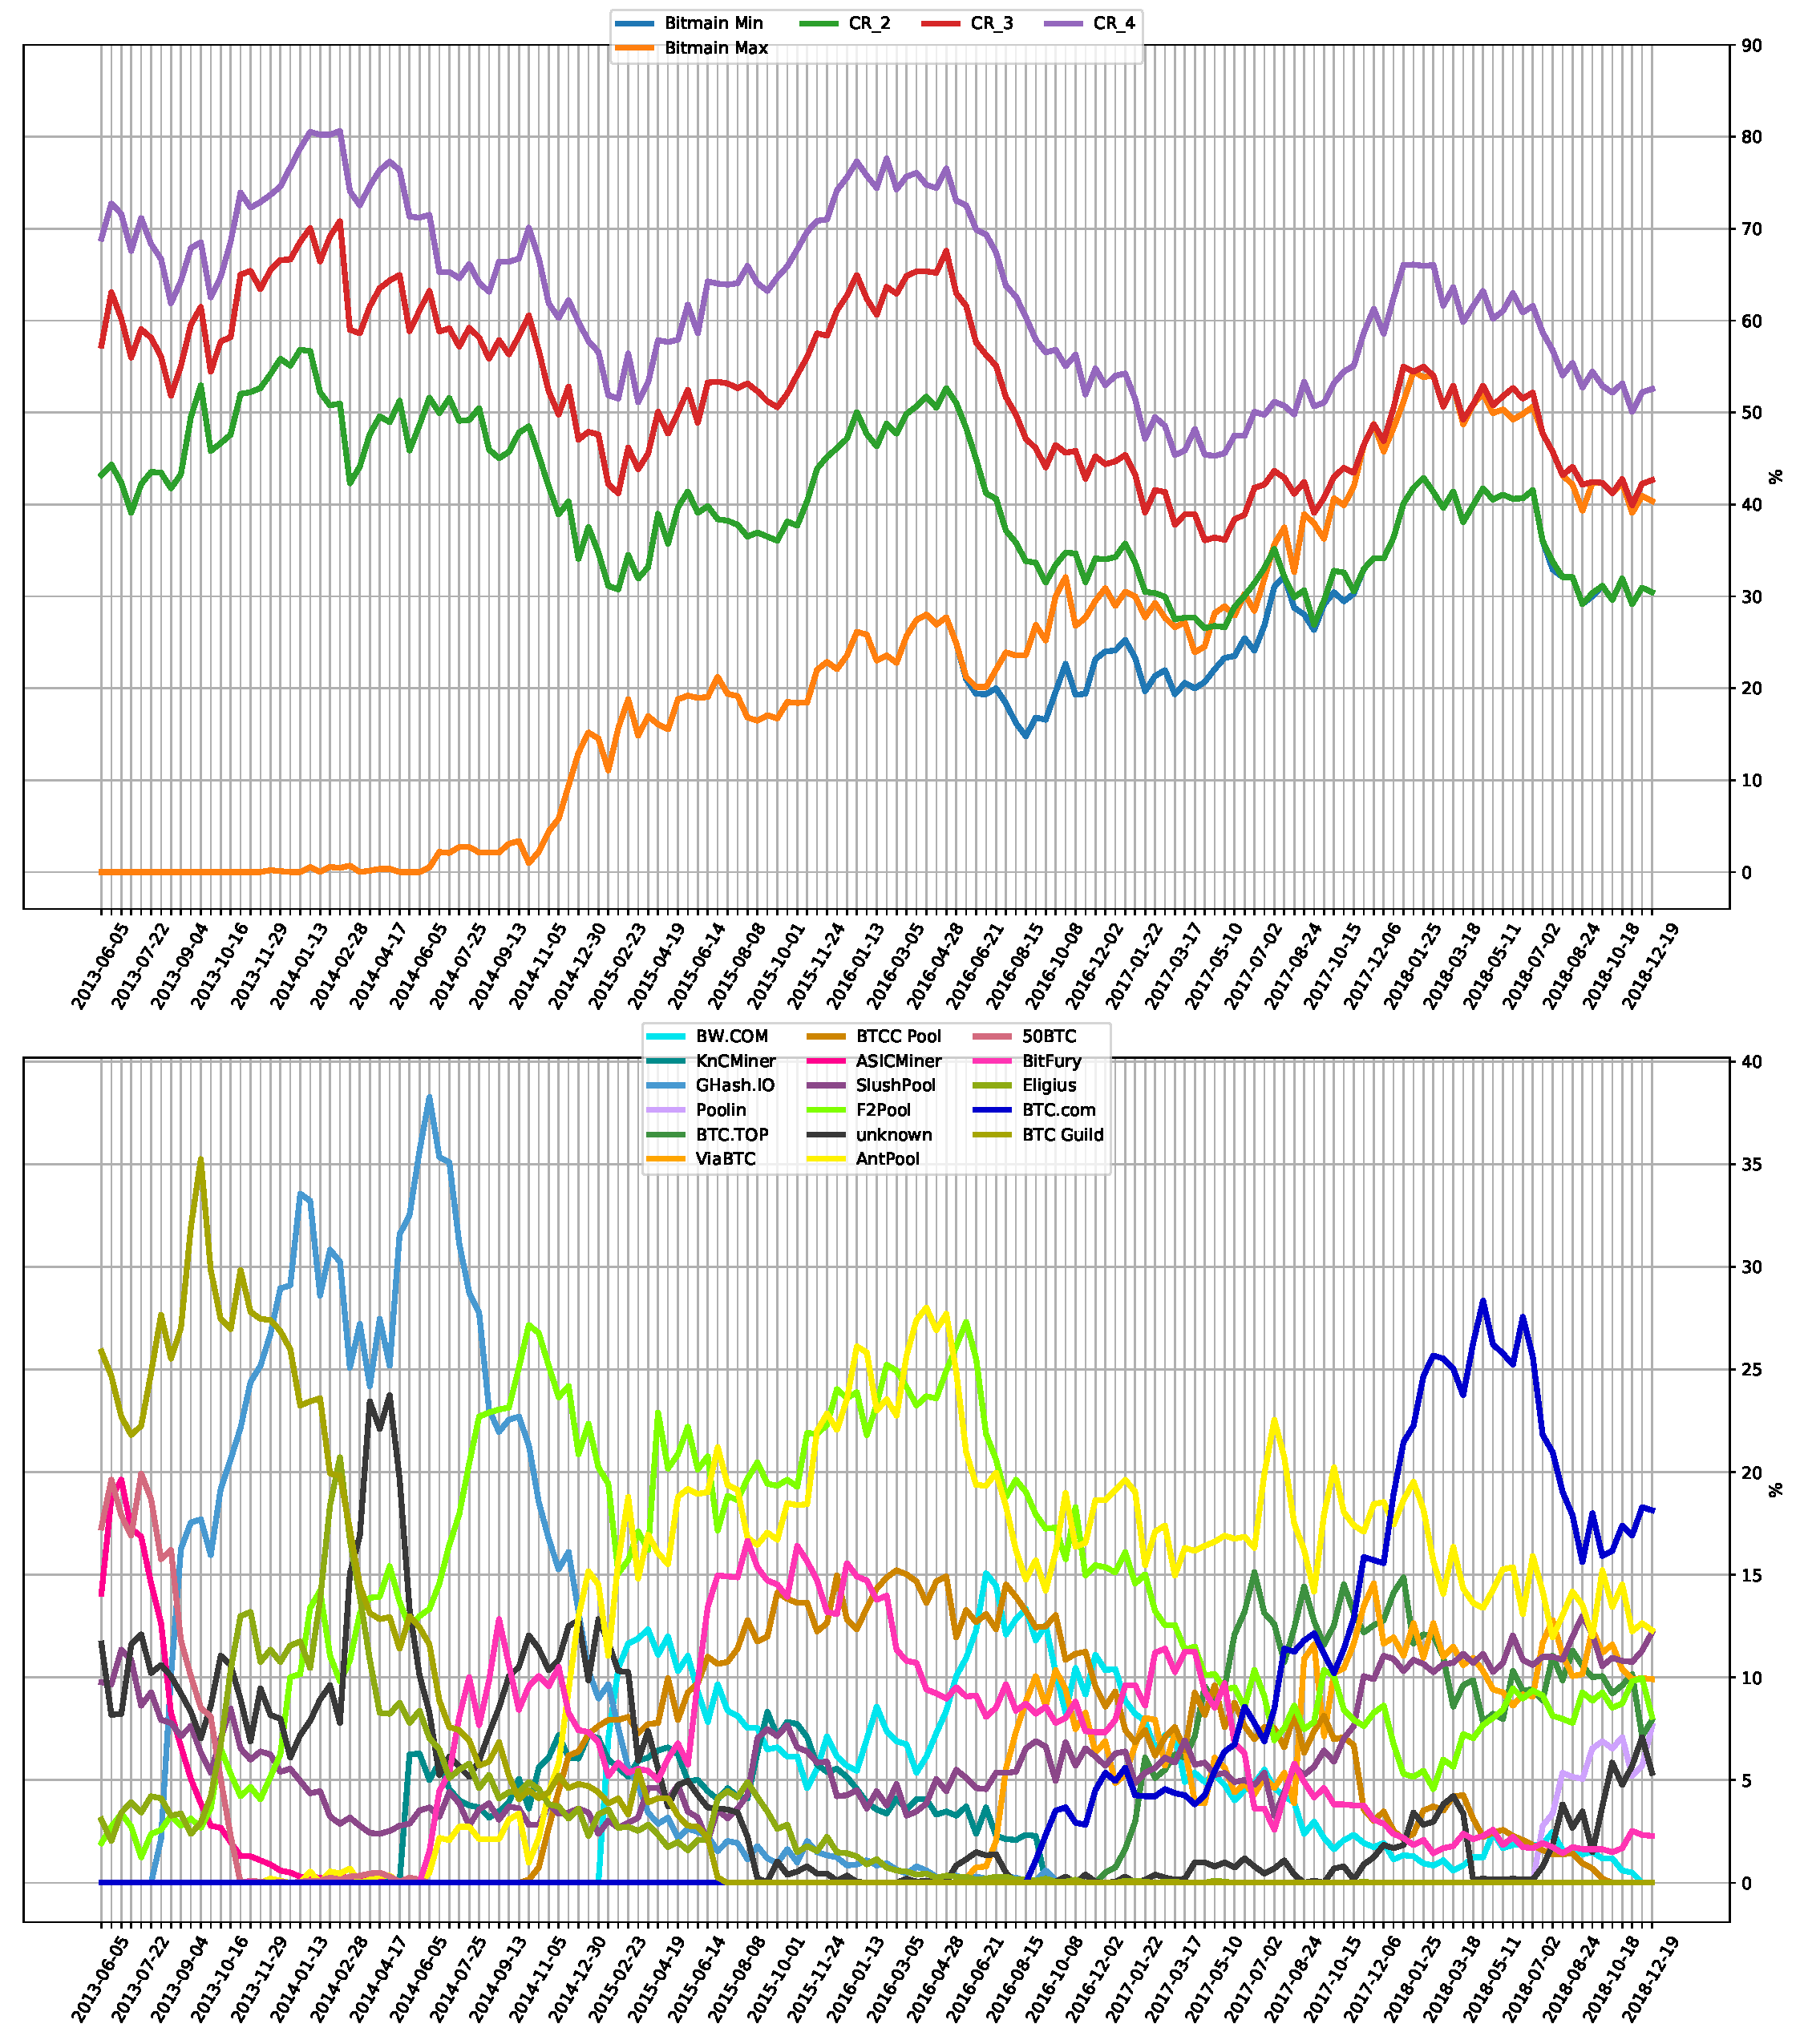
\includegraphics[width=.6\textwidth]{images/mining_distribution_157.pdf}
        \caption{Concentration indeces and mining shares.} \label{fig:mining_distribution}
    \end{figure}
\end{frame}

\begin{frame}[fragile]{Pools Members | Results: Cross-Pool Mining}
    \begin{figure}
        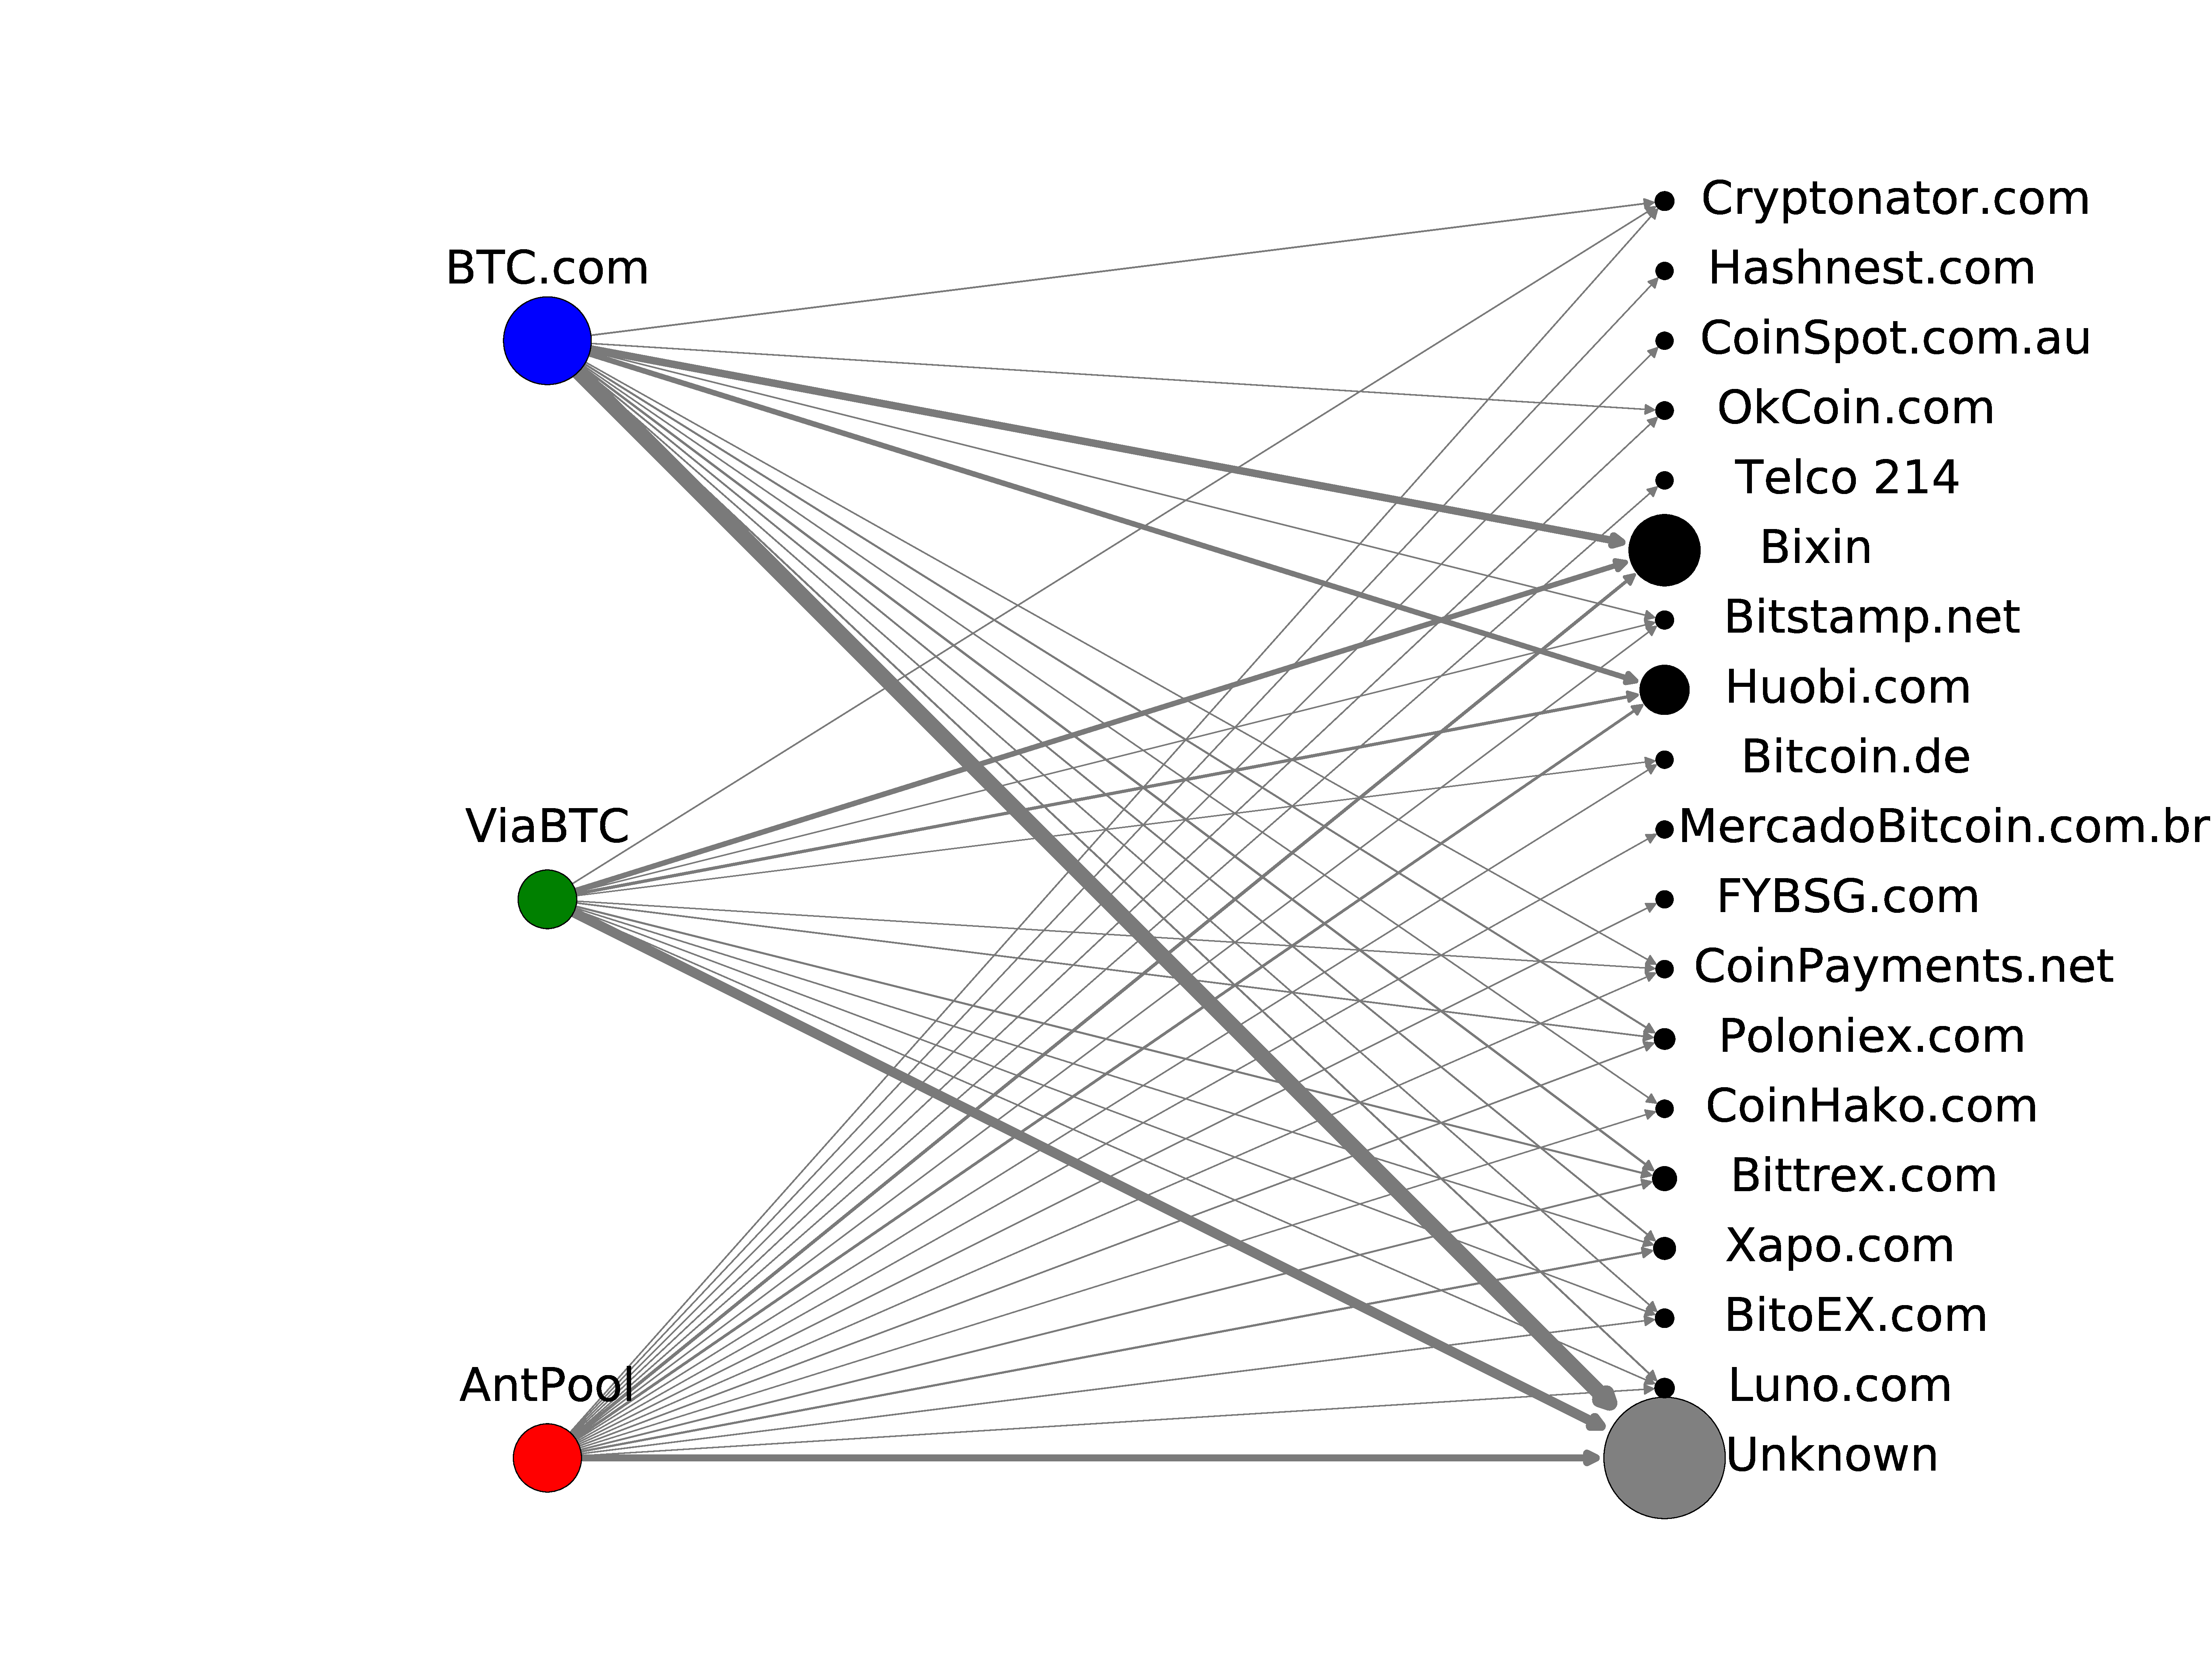
\includegraphics[width=0.7\columnwidth]{images/payments_graph_400.pdf}
        \caption{Flow of mining rewards from mining pools to their members. In black: wallet services and exchanges, in gray: unknown entities. This plot covers the top 400 clusters from each mining pool sorted by received BTC. \textit{Unknown} entities (1118) were combined into one node.}
        \label{fig:payment_graph}
    \end{figure}
\end{frame}

\begin{frame}[fragile]{Pools Members | Results: Cross-Pool Unknown Mining}
    \begin{table}[]
        \caption{Cross-pool mining of the ten largest unknown mining clusters sorted by total amount of BTC received by the three pools in the time period between block 510,000 and 514,032 ($\sim$ 4 weeks).}\label{table:crosspool_unknown_entities}

        \scalebox{0.8}{
            \begin{tabular}{@{}rrrrrrrrr@{}}
            \toprule
                       & \multicolumn{2}{c}{BTC.com}                         & \multicolumn{2}{c}{AntPool}                         & \multicolumn{2}{c}{ViaBTC}                          &                      &             \\ \cmidrule(lr){2-3} \cmidrule(lr){4-5} \cmidrule(lr){6-7}
            Cluster ID & \multicolumn{1}{c}{BTC} & \multicolumn{1}{c}{\%BTC} & \multicolumn{1}{c}{BTC} & \multicolumn{1}{c}{\%BTC} & \multicolumn{1}{c}{BTC} & \multicolumn{1}{c}{\%BTC} & \multicolumn{1}{c}{\begin{tabular}[c]{@{}c@{}}Mined\\BTC\end{tabular}} & \multicolumn{1}{c}{\begin{tabular}[c]{@{}c@{}}Total BTC\\Received\end{tabular}}     \\ \midrule
            327539880  & 409.34                  & 3.40                      & 122.10                  & 5.23                      & 258.55                  & 6.04                      & 789.99               & 521,939  \\
            324067473  & 295.02                  & 2.45                      & 90.44                   & 3.88                      & 189.15                  & 4.42                      & 574.61               & 3,756,583  \\
            350822682  & 244.77                  & 2.03                      & 9.29                    & 0.40                      & 182.92                  & 4.27                      & 436.98               & 110,566 \\
            350824718  & 244.67                  & 2.03                      & 65.65                   & 2.81                      & 46.20                   & 1.08                      & 356.52               & 112,680 \\
            333653856  & 153.02                  & 1.27                      & 54.02                   & 2.31                      & 83.60                   & 1.95                      & 290.63               & 130,680   \\
            372448840  & 181.10                  & 1.50                      & 33.64                   & 1.44                      & 55.73                   & 1.30                      & 270.48               & 882,713  \\
            234254928  & 93.31                   & 0.77                      & 27.18                   & 1.16                      & 58.68                   & 1.37                      & 179.17               & 905,101   \\
            249123673  & 15.63                   & 0.13                      & 0.40                    & 0.02                      & 107.23                  & 2.50                      & 123.26               & 6,812,938 \\
            349962609  & 8.67                    & 0.07                      & 39.01                   & 1.67                      & 19.74                   & 0.46                      & 67.41                & 1,173,892 \\
            311503667  & 38.94                   & 0.32                      & 7.47                    & 0.32                      & 7.77                    & 0.18                      & 54.18                & 486,338 \\
            \bottomrule
            \end{tabular}
        }
    \end{table}
\end{frame}

\begin{frame}[fragile]{Payout Patterns | Methodology}
    \begin{algorithm}[H]
        \caption{Find payout patterns in BTC.com, AntPool and ViaBTC.}\label{algo:blocks_addresses}
        \begin{algorithmic}[1]
            \For{each pool}
                \For{each mined block}
                    \State get coinbase flow of block
                    \State compute number of addresses at each step of the coinbase flow
                    \State save results
                \EndFor
                \State plot data and look for common patterns among flows
            \EndFor
        \end{algorithmic}
    \end{algorithm}
\end{frame}

\begin{frame}[fragile]{Payout Patterns | Methodology}
    \begin{figure}
        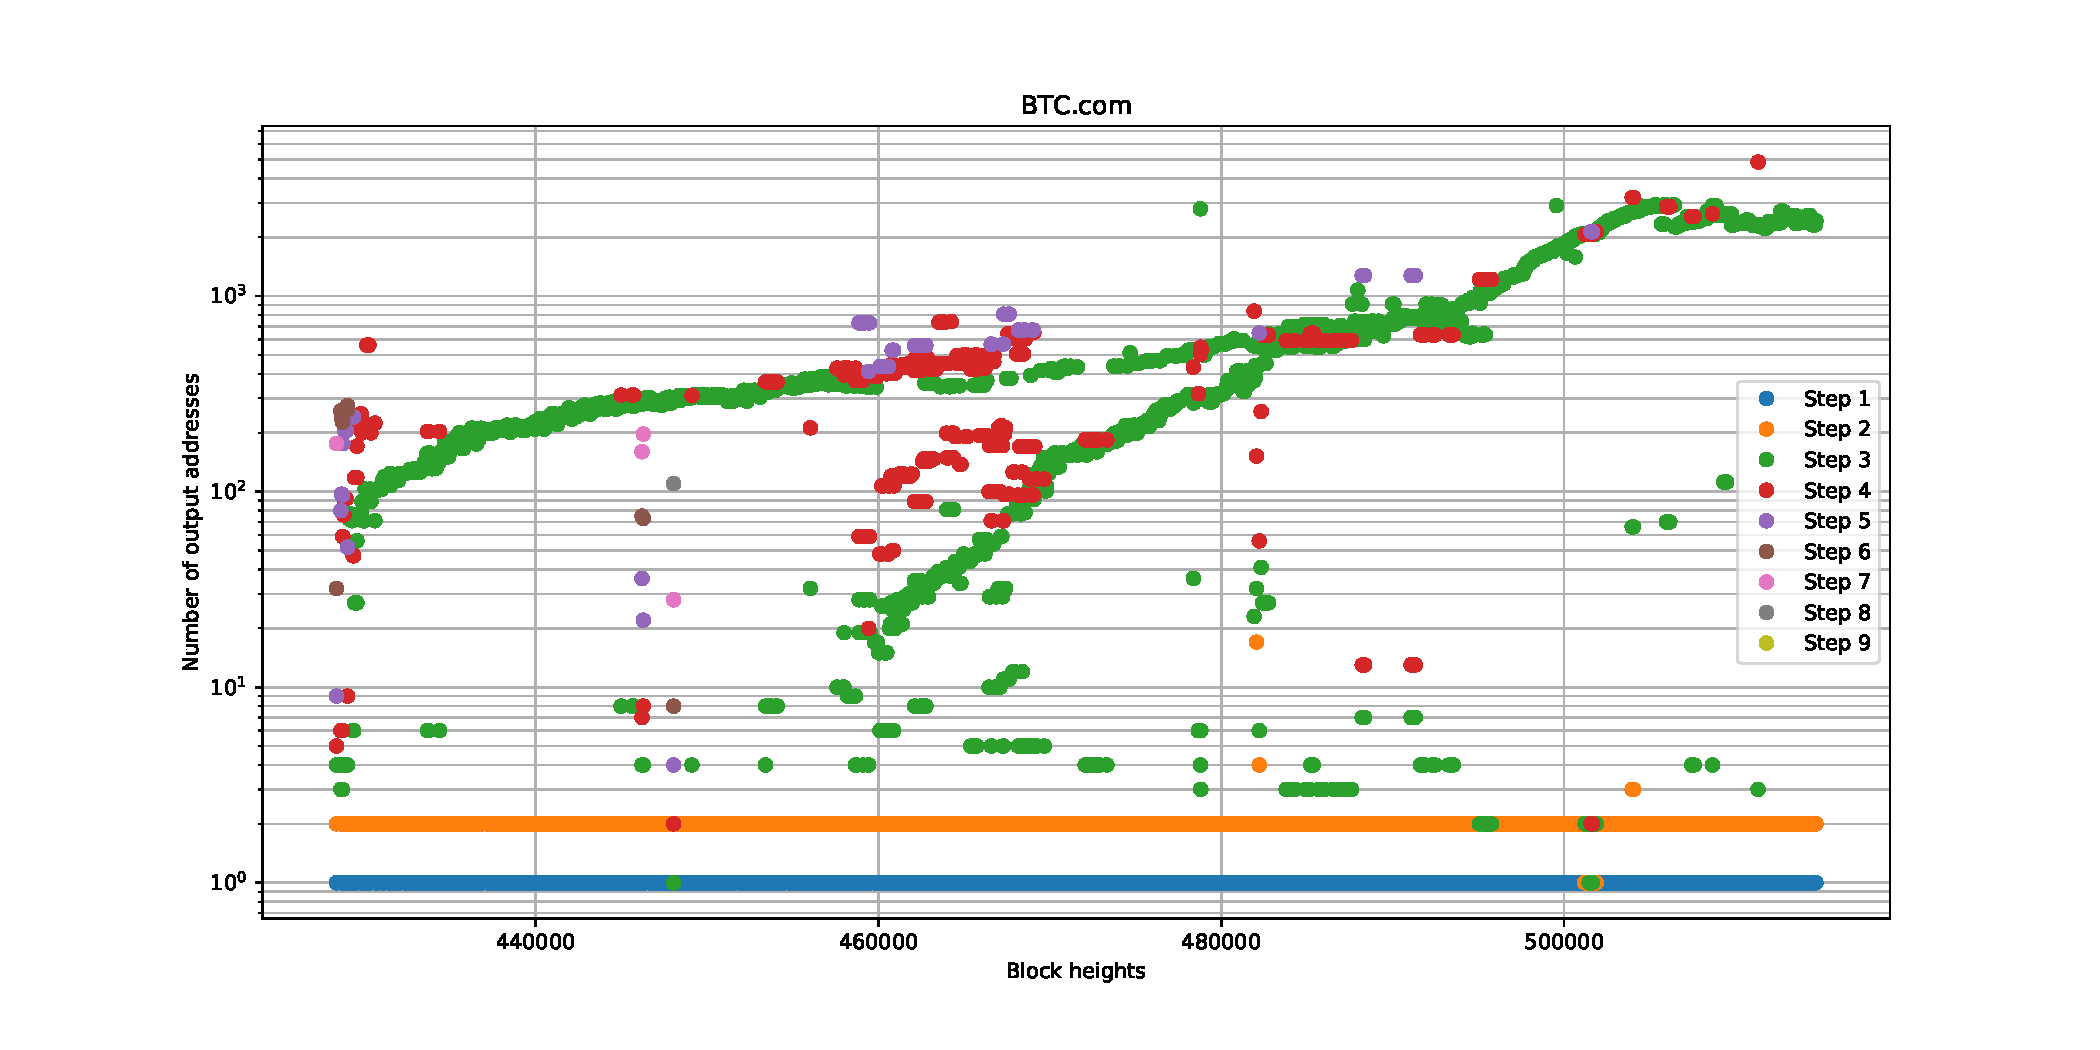
\includegraphics[width=\textwidth]{images/payout_trend_BTC_com.pdf}
        \caption{Payout trend for BTC.com} \label{fig:payout_trend_BTCcom}
    \end{figure}
\end{frame}

% \begin{frame}[fragile]{Appendix}
% % number of addresses per step 
%     \begin{figure}
%         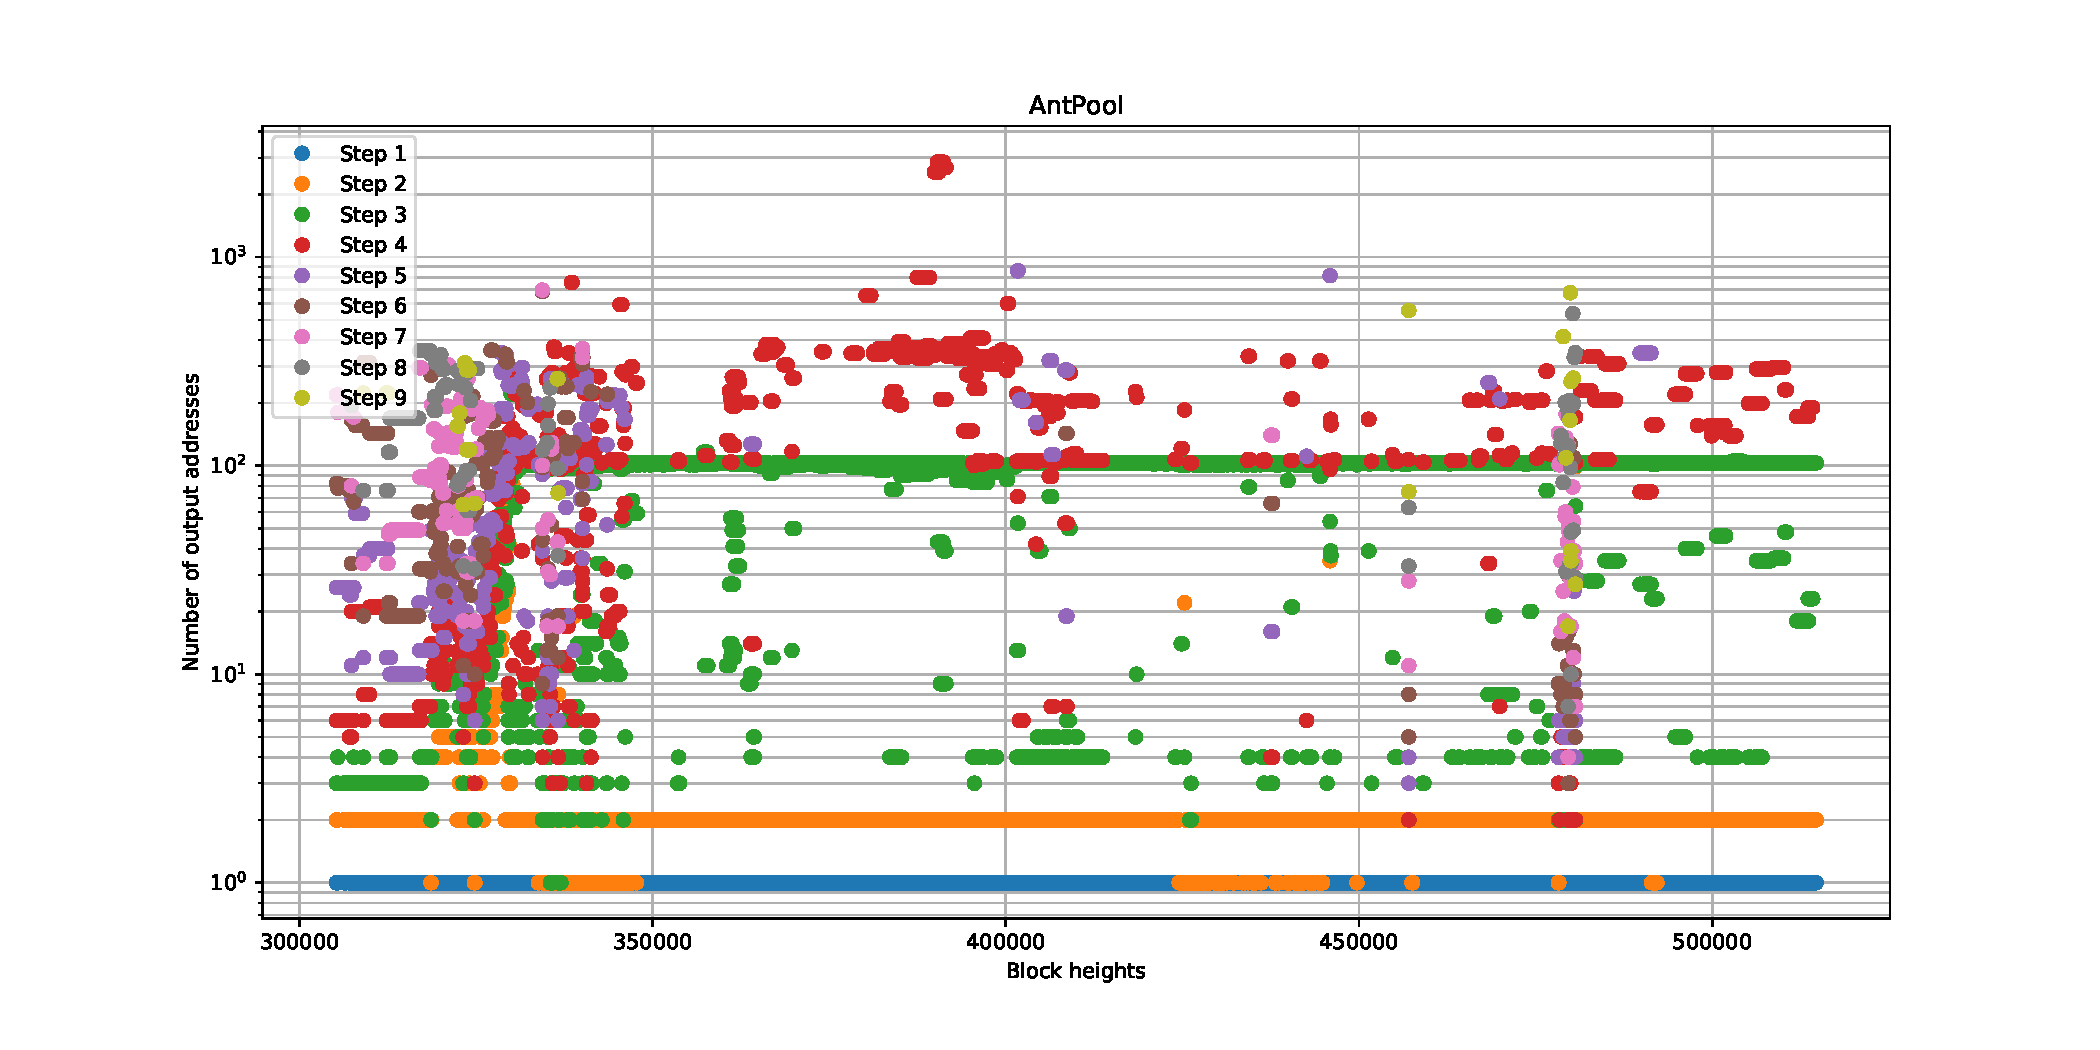
\includegraphics[width=0.8\textwidth]{images/payout_trend_AntPool.pdf}
%         \caption{Payout trend for AntPool} \label{fig:payout_trend_AntPool}
%     \end{figure}
% \end{frame}

% \begin{frame}[fragile]{Appendix}
% % number of addresses per step 
%     \begin{figure}
%         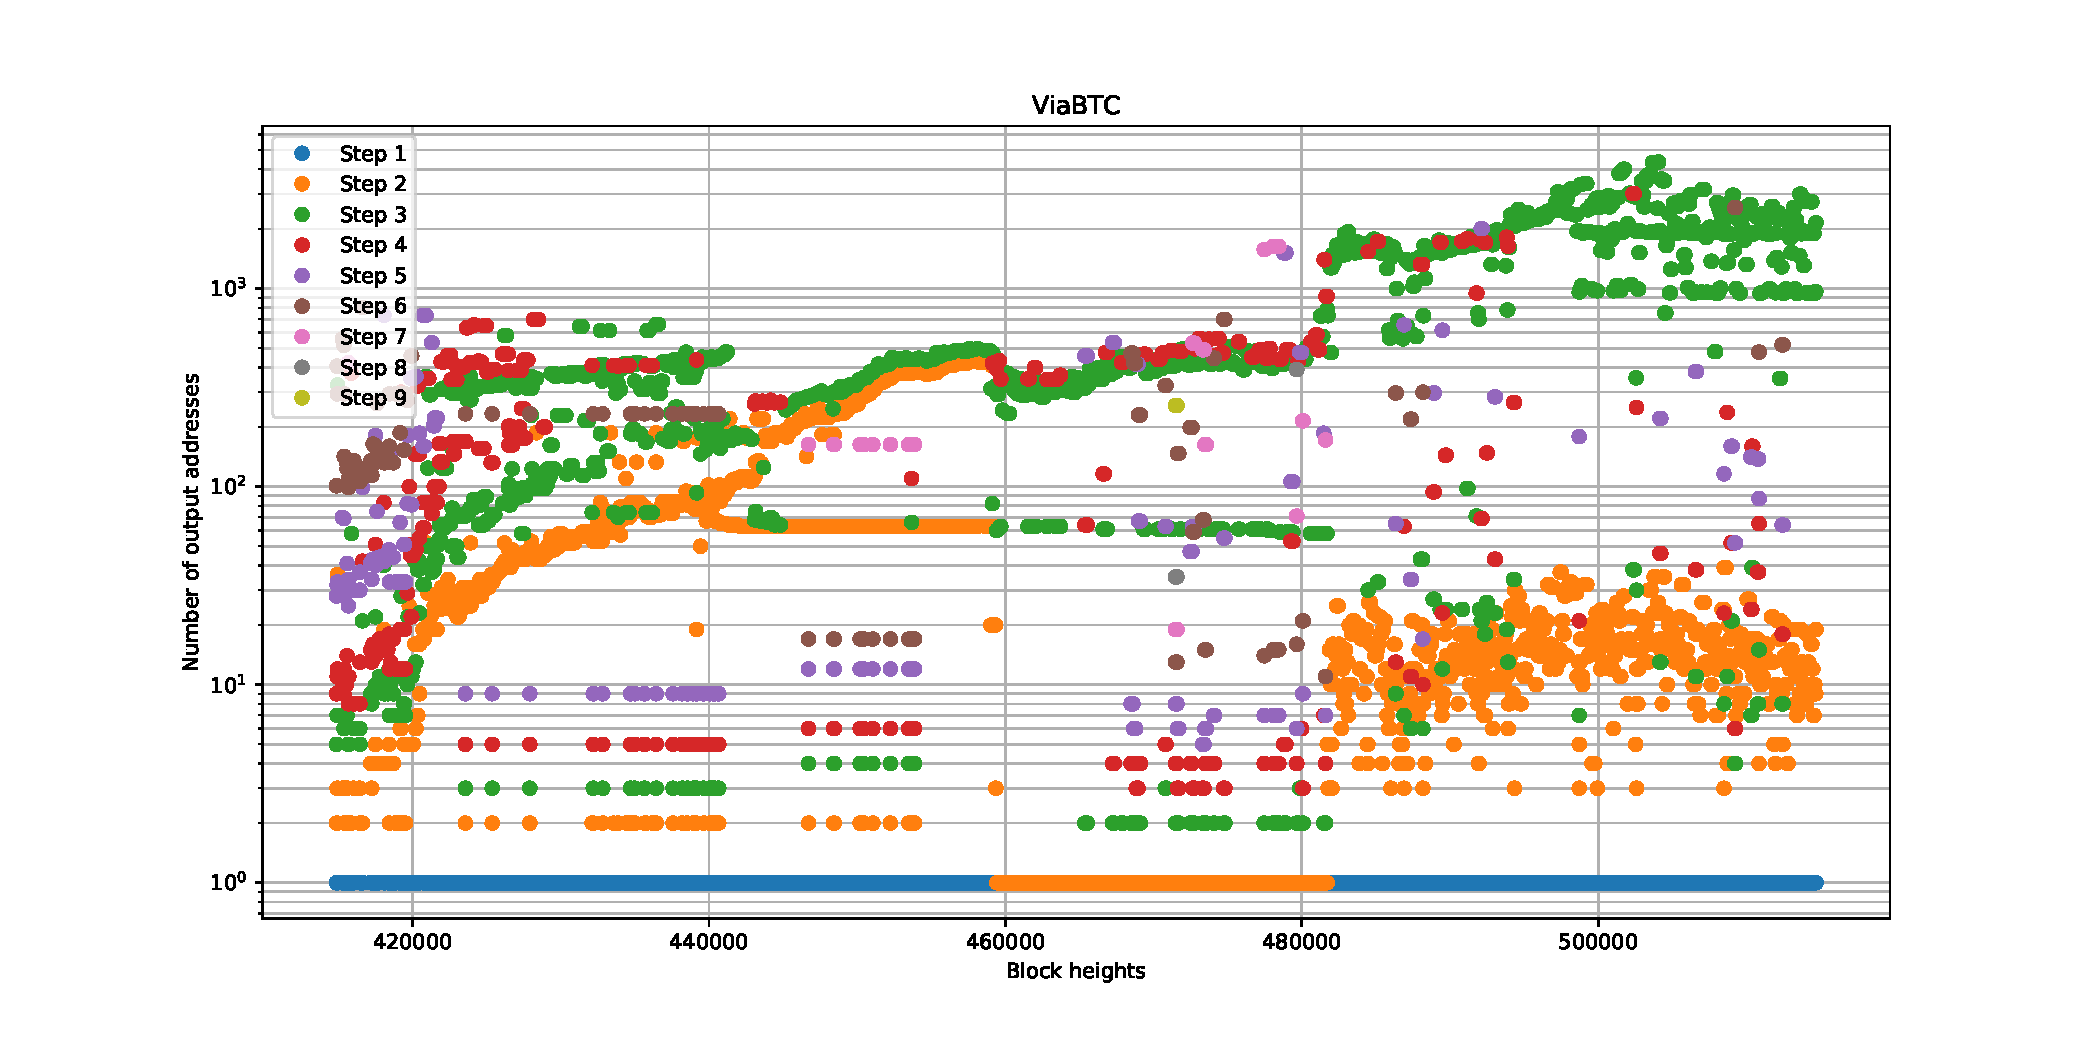
\includegraphics[width=0.8\textwidth]{images/payout_trend_ViaBTC.pdf}
%         \caption{Payout trend for ViaBTC} \label{fig:payout_trend_ViaBTC}
%     \end{figure}
% \end{frame}


\end{document}
